\chapter{Bias, Variance, and Ensembling}

A model is trained on the basis of a specific training dataset containing a finite number of instances. Each training set is only one of the possible realizations of the universe of data obtained through empirical measurements, so different training sets can provide different estimates. When determining the error of a model, noise should be taken into consideration. This chapter will focus on the different aspects that influence the quality of the final model.

\section{Bias, Variance, Noise}

The expected error of the model at a point $x$ can be decomposed as:
\begin{itemize}
    \item \textbf{Bias}: it quantifies the inability of the model to accurately approximate the target function. It can be seen as an approximation error.

    \item \textbf{Variance}: it quantifies the variability of the response of the model for different realizations of the training data. It can be seen as an estimation error.

    \item \textbf{Noise}: it's a random error included in a label in the training set, caused by imperfect measurements. It's irreducible, since it does not depend on the model.
\end{itemize}

Assume we have a regression task, where the target function is $y$ and we use the squared error loss $L_2$. Our training set is TR = $< X, y >$, where $y = f(x) + \epsilon$, and $\epsilon$ is Gaussian noise with 0 mean and standard deviation $\sigma$.

We fit a linear hypothesis $h(x) = wx + w_0$ to minimize the SSE over the training data. We will have a systematic prediction error, since the model is not flexible enough to approximate certain target functions (e.g. second degree functions). Also, depending on the dataset, the $w$ parameters will be calculated differently.

So, given a new data point $x$, what is the expected prediction error? Assume that all the data points are drawn from a set of independent and identically distributed variables with the same probability distribution $P$. The goal is to compute, for any new $x$:
\begin{equation*}
    E_p [(y-h(x))^2] \,,
\end{equation*}
where $y$ is the value of $x$ that can be found in a dataset, and the expectation is over all training sets drawn according to $P$.

Let $Z$ be a random variable with possible values $z_i, \, i = 1 \dots l$ and probability sitribution $P(Z)$. Its \textbf{expected value (mean)} is:
\begin{equation*}
    \Bar{Z} = E_p[Z] = \sum_{i=1}^l z_iP(z_i)
\end{equation*}
If $Z$ is continuous, the sum is replaced with an integral, and the distribution function by a density one. The \textbf{variance} of $Z$ is:
\begin{equation*}
    Var[Z] = E[(Z - \Bar{Z})^2] = E[Z^2] - \Bar{Z}^2 \,.
\end{equation*}
The proof of this last equality is the following:
\begin{gather*}
    Var[Z] = E[(Z - \Bar{Z})^2] = \sum_{i=1}^l (z_i - \Bar{Z})^2 P(z_i) = \\
    = \sum_{i=1}^l (z_i^2 - 2 z_i \Bar{Z} + \Bar{Z}^2) P(z_i) = \sum_{i=1}^l z_i^2 P(z_i) - \sum_{i=1}^l 2 z_i \Bar{Z} P(z_i) + \sum_{i=1}^l \Bar{Z}^2 P(z_i) = \\
     = E[Z^2] - 2\Bar{Z} \sum_{i=1}^l z_i P(z_i) + \Bar{Z}^2 \sum_{i=1}^l P(z_i) = E[Z^2] - 2 \Bar{Z} \Bar{Z} + \Bar{Z}^2 \dot 1 = \\
     = E[Z^2] - 2 \Bar{Z}^2 + \Bar{Z}^2 = E[Z^2] - \Bar{Z}^2 = Var[Z]
\end{gather*}
We will use the form $E[Z^2] = \Bar{Z}^2 + Var[Z]$ (variance lemma).

The error can be rewritten as:
\begin{equation*}
    E_p[(y - h(x))^2] = E_p[h(x)^2 - 2yh(x) + y^2] = E_p[h(x)^2] + E_p[y^2]] - 2E_p[y]E_p[h(x)]
\end{equation*}
Let $\Bar{h}(x) = E_p[h(x)]$ be the mean prediction of the hypothesis at $x$ when $h$ is trained on data drawn from $P$. Using the variance lemma defined above, we can rewrite the squared error as:
\begin{gather*}
    E_p[(y - h(x))^2] = \Bar{h}(x)^2 + E_p[(h(x) - \Bar{h}(x))^2] + f(x)^2 + E_p[(y - f(x))^2] - 2f(x)\Bar{h(x)} = \\
    = E_p[(h(x) - \Bar{h}(x))^2] + \Bar{h}(x)^2 - 2f(x)E_p[h(x)] + f(x)^2 + E_p[(y - f(x))^2] = \\
    = E_p[(h(x) - \Bar{h}(x))^2] + \textbf{(variance)}\\
    + (\Bar{h(x)} - f(x))^2 + \textbf{(bias$^2$)} \\
    + E_p[(y - f(x))^2] = \textbf{(noise$^2$)} \\
    = Var[h(x)] + Bias[h(x)]^2 + E_p[\epsilon^2]
\end{gather*}
(the mean of $y$ is $f(x)$).

\subsection{Regularization}

Recall how we implemented regularization to calculate the loss function:
\begin{equation*}
    Loss(w) = \sum_p (d_p - o(x_p))^2 + \lambda \|w\|^2
\end{equation*}
By varying the value of the regularization hyperparameter $\lambda$, we ca obtain more or less complex solutions. Consider the following graphical examples to understand how it affects bias and variance of the model; the training sets here are taken from a sinusoidal distribution.

\begin{figure}[H]
    \centering
    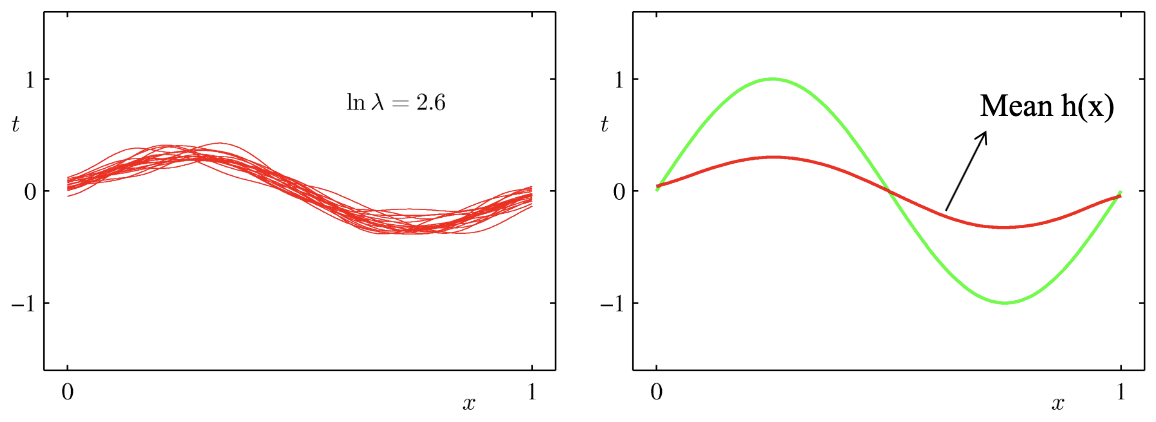
\includegraphics[width=0.9\textwidth]{img/BiasVar1.png}
    \caption{High lambda, high bias, low variance. Not too dependent on data, but the model is too rigid. The model underfits the data.}
\end{figure}
\begin{figure}[H]
    \centering
    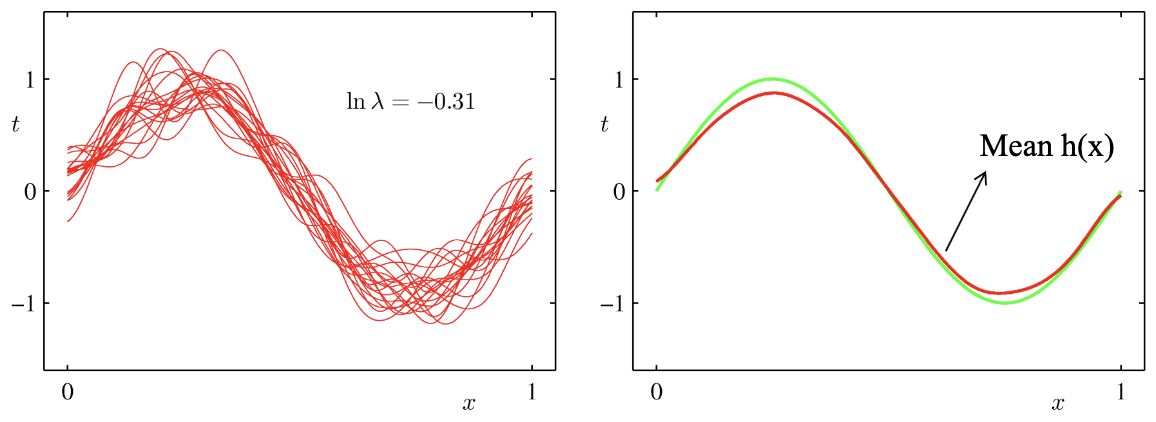
\includegraphics[width=0.9\textwidth]{img/BiasVar2.png}
    \caption{Low lambda, low bias, high variance. The model is more dependent on training data, but approximates better.}
\end{figure}
\begin{figure}[H]
    \centering
    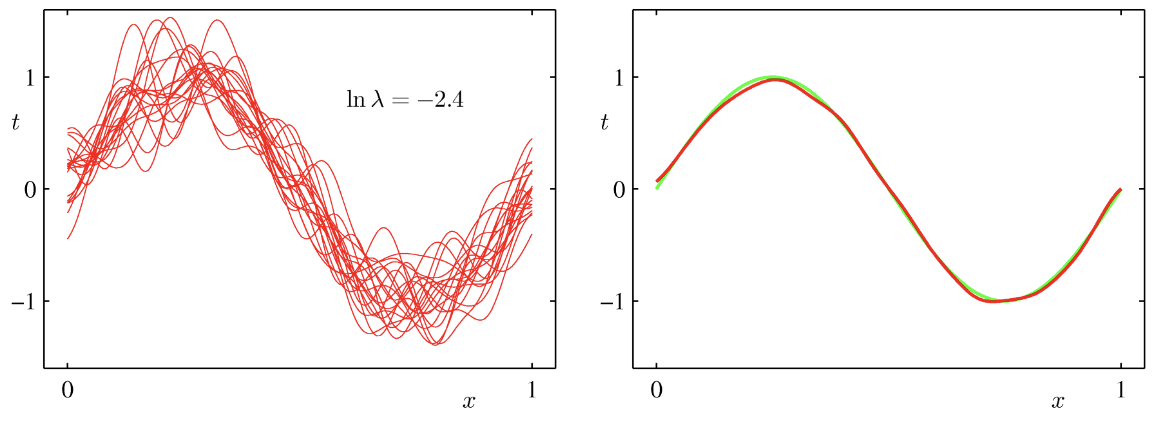
\includegraphics[width=0.9\textwidth]{img/BiasVar3.png}
    \caption{Very low lambda, very low bias, very high variance. Final hypothesis may produce an high test error. The model overfits the data.}
\end{figure}
This highlights once again how the goal of model selection is to find the best trade-off between model complexity (bias) and training error (variance).

\section{Ensemble learning}

Ensemble learning estimates the output of an instance by considering the prediction of multiple models trained differently instead of just one.

The simplest case is \textbf{voting}. All models are trained on the same training set. For regression, the simple average committee of the models is calculated:
\begin{equation*}
    o(x) = \dfrac{1}{K} \sum_{k=1}^K h_k(x)
\end{equation*}
The square error of a committee is less or equal than the mean of the square error. For classification, we use different classifiers and take the majority vote (or the instance is classified after calculating the mean of the continuous outputs).

Another scheme is \textbf{bagging} (also called \textbf{bootstrap aggregating}). $K$ models are trained on different subsets of the training set, and each training is differentiating using bootstrap (so resampling with replacement). For regression, the final prediction will be the mean, while for classification we consider the majority vote.

If models have the same errors, however, we will not have any advantage in using ensembling. A solution is \textbf{boosting}: we first differentiate each training in order concentrating on errors, so we give more weight to ``difficult'' instances, such as ones that get misclassified by the previous classifier. The results are then combined in the output weights. If not stopped, boosting will learn to classify correctly all training instances, even when given a set of weak learners that are barely better than a random guesser. Even if bias is reduced, variance does not increase, so it resists well to overfitting (although it's not immune). However, it's sensitive to noisy data, since it will be deemed ``difficult'' and therefore receive an heavier weight.

